%; whizzy chapter -dvi
% -initex iniptex -latex platex -format platex -bibtex jbibtex -fmt fmt
% $B0J>e(B whizzytex $B$r;HMQ$9$k>l9g$N@_Dj!#(B

%     Tokyo Debian Meeting resources
%     Copyright (C) 2012 Junichi Uekawa
%     Copyright (C) 2011, 2015, 2020 Nobuhiro Iwamatsu

%     This program is free software; you can redistribute it and/or modify
%     it under the terms of the GNU General Public License as published by
%     the Free Software Foundation; either version 2 of the License, or
%     (at your option) any later version.

%     This program is distributed in the hope that it will be useful,
%     but WITHOUT ANY WARRANTY; without even the implied warranty of
%     MERCHANTABILITY or FITNESS FOR A PARTICULAR PURPOSE.  See the
%     GNU General Public License for more details.

%     You should have received a copy of the GNU General Public License
%     along with this program; if not, write to the Free Software
%     Foundation, Inc., 51 Franklin St, Fifth Floor, Boston, MA  02110-1301 USA

%  preview (shell-command (concat "evince " (replace-regexp-in-string "tex$" "pdf"(buffer-file-name)) "&"))

%%$B$3$3$+$i%X%C%@3+;O!#(B

\documentclass[mingoth,a4paper]{jsarticle}
\usepackage{monthlyreport}
% $BF|IU$rDj5A$9$k!"Kh7nJQ$o$j$^$9!#(B
\newcommand{\debmtgyear}{2020}
\newcommand{\debmtgmonth}{5}
\newcommand{\debmtgdate}{16}
% started from zero:
% (let ((year 2013) (month 7)) (+ (* (- year 2005) 12) month -1))
\newcommand{\debmtgnumber}{185}

% Needed to import pandoc-generated LaTeX documents.
% See https://stackoverflow.com/questions/40438037/tightlist-error-using-pandoc-with-markdown
\providecommand{\tightlist}{%
  \setlength{\itemsep}{0pt}\setlength{\parskip}{0pt}}

% tikz picture $B$N0Y$N%^%/%m@_Dj(B
\usepackage[dvipdfmx]{graphicx}
\usepackage{tikz}

\begin{document}

\begin{titlepage}
\thispagestyle{empty}
% $B%?%$%H%k%Z!<%8(B:$BJT=8I,MW$JItJ,$O:G=i$N%^%/%m$KHt$P$9$3$H(B

\vspace*{-2cm}
$BBh(B\debmtgnumber{}$B2s(B $BEl5~%(%j%"(B Debian $BJY6/2q;qNA(B\\
\hspace*{-2cm}

\includegraphics{image2012-natsu/dotdeb.pdf}\\
\hfill{}\debmtgyear{}$BG/(B\debmtgmonth{}$B7n(B\debmtgdate{}$BF|(B

% $B$3$3$O%"%C%W%G!<%H$9$k$3$H(B
% $BA43QJ8;z$K$7$J$$$H%U%)%s%H$N%5%$%:$,9g$o$J$$$N$GCm0U(B
\rotatebox{10}{\fontsize{30}{30} {\gt$B!!#a#p#t#l#yFC=8(B}}\\

\vspace*{-2cm}
\hfill{}
\includegraphics[height=6cm]{image200502/openlogo-nd.eps}
\end{titlepage}

\newpage

\begin{minipage}[b]{0.2\hsize}
 \definecolor{titleback}{gray}{0.9}
 \colorbox{titleback}{\rotatebox{90}{\fontsize{80}{80} {\gt $B%G%S%"%sJY6/2q(B} }}
\end{minipage}
\begin{minipage}[b]{0.8\hsize}
\hrule
\vspace{2mm}
\hrule
\begin{multicols}{2}
\tableofcontents
\end{multicols}
\vspace{2mm}
\hrule
\end{minipage}

\dancersection{$B:G6a$N(BDebian$B4XO"$N%_!<%F%#%s%0Js9p(B}{$B?yK\!!E5=<(B}

\subsection{2020$BG/(B4$B7nEY(B $BEl5~%(%j%"!&4X@>9gF1(BDebian$BJY6/2q(B}

2020$BG/(B4$B7n(B18$BF|(B($BEZ(B)$B$KEl5~%(%j%"(BDebian$BJY6/2q$H4X@>(BDebian$BJY6/2q$N9gF1$G%*%s%i%$%s$K$h$k(BDebian$BJY6/2q$r3+:E$7$^$7$?!#;22C<T$O(B35$BL>$G$7$?!#%;%_%J!<H/I=$r(B2$B$D9T$$$^$7$?!#(B


$B%;%_%J!<!V(BWireguard $B<BA)F~Lg!W$H$$$&I=Bj$G@>;3OB9-$5$s$,H/I=$7$^$7$?!#(BWireguard$B$O(BVPN$B@\B3$9$k%"%W%j%1!<%7%g%s$G$"$j!"%5!<%P$H%/%i%$%"%s%H$r%9%?!<7?$G@\B3$9$k9=@.$NB>!"%a%C%7%e7?$N@\B3$b2DG=$H$N@bL@$G$7$?!#(Blinux-5.6$B$h$j8E$$%+!<%M%k$N>l9g$O%+!<%M%k%b%8%e!<%k$r(BDKMS$B$G%S%k%I$7$FMxMQ$7!"(Blinux-5.6$B0J9_$G$O%+!<%M%k$K%^!<%8$5$l$F$$$k$J$I:G?7$NF08~$N@bL@$,$"$j$^$7$?!#$^$?!"<A5?1~Ez$G$O(BOpenVPN$B$HBPHf$9$k<ALd$,$"$j$^$7$?!#(B


$B%;%_%J!<!V(BJitsi$B$r;H$C$?%S%G%*2q5D%5!<%P$N:n$jJ}!W$H$$$&I=Bj$G?yK\E5=<$5$s$,H/I=$7$^$7$?!#(B2020$BG/(B3$B7n$K3+:E$7$?(BDebian$BJY6/2q$O%$%s%?!<%M%C%H$rMQ$$$?%S%G%*2q5D7A<0$G3+:E$7$F$*$j!"$=$N$H$-$KMxMQ$7$?%"%W%j%1!<%7%g%s$G$"$k(BJitsi$B!J%8%C%A!<!K$r@bL@$7$^$7$?!#(BJitsi$B$r(BGCP$B$N%5!<%P$K%$%s%9%H!<%k$7$F;H$($k$h$&$K$9$k<j=g$N@bL@!"@_Dj$N%+%9%?%^%$%:J}K!$N>R2p!"(B2020$BG/(B3$B7n$K3+:E$7$?(BDebian$BJY6/2q$N$H$-$N%5!<%P$N(BCPU$BMxMQN($H%H%i%U%#%C%/%0%i%U$r>R2p$7$^$7$?!#(B


\dancersection{$B;vA02]Bj(B}{$B?yK\!!E5=<(B}

$B:#2s$N;vA02]Bj$O0J2<$G$9!#(B

\begin{enumerate}
\item aptly $B$O$4B8$8$G$9$+(B
\end{enumerate}

%$B$3$N2]Bj$KBP$7$FDs=P$$$?$@$$$?FbMF$O0J2<$G$9!#(B

\begin{multicols}{2}
{\small
\begin{prework}{ dictoss }
  \begin{enumerate}
  \item $BCN$i$J$$(B
  \end{enumerate}
\end{prework}

\begin{prework}{ yy\_y\_ja\_jp }
  \begin{enumerate}
  \item $BCN$i$J$$(B
  \end{enumerate}
\end{prework}

\begin{prework}{ uwabami }
  \begin{enumerate}
  \item $BCN$C$F$$$k$,!";H$C$?$3$H$O$J$$(B
  \end{enumerate}
\end{prework}

\begin{prework}{ yosuke\_san }
  \begin{enumerate}
  \item $BCN$i$J$$(B
  \end{enumerate}
\end{prework}

\begin{prework}{ $B$"(B (cpa119) }
  \begin{enumerate}
  \item $BCN$i$J$$(B
  \end{enumerate}
\end{prework}

\begin{prework}{ MasanoriYoshida }
  \begin{enumerate}
  \item $BCN$i$J$$(B
  \end{enumerate}
\end{prework}

\begin{prework}{ NOKUBI Takatsugu (knok) }
  \begin{enumerate}
  \item $BCN$i$J$$(B
  \end{enumerate}
\end{prework}

\begin{prework}{ su\_do }
  \begin{enumerate}
  \item $BCN$i$J$$(B
  \end{enumerate}
\end{prework}

\begin{prework}{ TANIGUCHI Takaki (takaki\_t) }
  \begin{enumerate}
  \item $BCN$i$J$$(B
  \end{enumerate}
\end{prework}

\begin{prework}{ noncatalyst }
  \begin{enumerate}
  \item $BCN$i$J$$(B
  \end{enumerate}
\end{prework}

\begin{prework}{ kozo2 }
  \begin{enumerate}
  \item $BCN$i$J$$(B
  \end{enumerate}
\end{prework}

\begin{prework}{ matoken }
  \begin{enumerate}
  \item $BCN$C$F$$$k$,!";H$C$?$3$H$O$J$$(B
  \end{enumerate}
\end{prework}

\begin{prework}{ $B%W%i%$%K%s%0!!%N%k%Y%k%H(B (norbu) }
  \begin{enumerate}
  \item $B;H$C$?$3$H$,$"$k(B
  \end{enumerate}
\end{prework}

\begin{prework}{ Katsuki Kobayashi (rarewin) }
  \begin{enumerate}
  \item $BCN$i$J$$(B
  \end{enumerate}
\end{prework}

\begin{prework}{ koedoyoshida }
  \begin{enumerate}
  \item $BCN$i$J$$(B
  \end{enumerate}
\end{prework}

\begin{prework}{ $B1]??<#(B (enoki) }
  \begin{enumerate}
  \item $BCN$i$J$$(B
  \end{enumerate}
\end{prework}

\begin{prework}{ daromart }
  \begin{enumerate}
  \item $BCN$C$F$$$k$,!";H$C$?$3$H$O$J$$(B
  \end{enumerate}
\end{prework}

\begin{prework}{ Incognito (cyberconn) }
  \begin{enumerate}
  \item $BCN$i$J$$(B
  \end{enumerate}
\end{prework}

\begin{prework}{ ipv6waterstar }
  \begin{enumerate}
  \item $BCN$C$F$$$k$,!";H$C$?$3$H$O$J$$(B
  \end{enumerate}
\end{prework}

\begin{prework}{ Kazuhiro NISHIYAMA (znz) }
  \begin{enumerate}
  \item $BCN$i$J$$(B
  \end{enumerate}
\end{prework}

\begin{prework}{ Kouhei Maeda (mkouhei) }
  \begin{enumerate}
  \item $BCN$C$F$$$k$,!";H$C$?$3$H$O$J$$(B
  \end{enumerate}
\end{prework}

}
\end{multicols}

%\dancersection{Debian Trivia Quiz}{username}
%
%Debian$B$N:r:#$NOCBj$K$D$$$F$N(BQuiz$B$G$9!#(B
%
%$B:#2s$N=PBjHO0O$O(B\url{debian-devel-announce@lists.debian.org} $B$d(B \url{debian-news@lists.debian.org}$B$J$I$KEj9F$5$l$?FbMF$+$i$G$9!#(B
%
%\begin{multicols}{2}
%%; whizzy-master ../debianmeetingresume201211.tex
% $B0J>e$N@_Dj$r$7$F$$$k$?$a!"$3$N%U%!%$%k$G(B M-x whizzytex $B$9$k$H!"(Bwhizzytex$B$,MxMQ$G$-$^$9!#(B
%

\santaku
{DebConf13 $B$N3+:ECO$H3+:EF|$O!)(B}
{$BF|K\!"El5~ET(B 6$B7n(B20$BF|(B}
{$B%K%+%i%0%"(B $B%^%J%0%"(B 7$B7n(B8-14$BF|(B}
{$B%9%$%9!"%t%)!<%^%k%-%e(B 8$B7n(B11-18$BF|(B}
{3}
{$B%K%+%i%0%"$O(BDebConf12$B$N3+:ECO$G$9!#(B
DebConf13$B$O%9%$%9$N%-%c%s%WCO$G3+:E$G$9!#(B
6/20$B$O3'$5$sM=Dj$r6u$1$F$*$-$^$7$g$&!#(B}

\santaku
{$B@$3&$N(BWeb$B%5!<%P$G:G$b?M5$$N$"$k(BLinux $B%G%#%9%H%j%S%e!<%7%g%s(B(W3Techs$BD4$Y(B)$B$O!)(B}
{CentOS}
{Debian}
{Ubuntu}
{B}
{\url{http://w3techs.com/technologies/history_details/os-linux}$B$K7k2L$N%0%i%U$,$"$j$^$9!#(B
$B8=:_(B Linux $B$r;HMQ$7$F$$$k(B web $B%5!<%P$N(B 32.9\% $B$,(B Debian $B$rMxMQ$7$F$*$j!"$=$N3d9g$O8=:_$bA}2C$rB3$1$F$$$k$=$&$G$9!#(B}

\santaku
{Debian $B%+!<%M%k%A!<%`$N%a%s%P!<$G$"$j!"(Bkernel.org $B$N(B 3.2.y $B0BDjHG7ONs$N%a%s%F%J$G$b$"$k(B Ben Hutchings $B$5$s$,<!4|(B Debian $B0BDjHG$H0l=o$K=P2Y$5$l$k(B Linux $B%+!<%M%k$K(B (3.2 $B7ONs$N(B mainline $B$K$OL5$$(B) $BDI2C5!G=$,Ek:\$5$l$kM=Dj$G$"$k$H=R$Y$F$$$^$9!#(B
$BB?$/$NDI2CE@$NCf$K4^$^$l$J$$$b$N$O2?!)(B}
{PREEMPT\_RT}
{Hyper-V guest drivers$B$N6/2=(B}
{ARM64/AArch64$B%"!<%-%F%/%A%c%5%]!<%H(B}
{C}
{Hyper-V guest drivers$B$O(Bmainline kernel$B$G(B3.2$B$K$b4^$^$l$F$$$^$9$,!"$h$j2~A1$5$l$?(B3.4$B$+$i$N=$@5$,F3F~$5$l$^$9!#(B
PREEMPT\_RT$B$O%O!<%I%j%"%k%?%$%`$r<B8=$9$k$?$a$N(BPatch$B!"(B
linux-image-rt-amd64 , linux-image-rt-686-pae $B$N(Bmetapackage$B$G;HMQ$G$-$^$9!#(B
$B?7$7$$(BARM 64$B%S%C%H%"!<%-%F%/%A%c%5%]!<%H$O(Bmainline kernel 3.7$B$+$i(B}

\santaku
{Wookey$B$5$s$,%"%J%&%s%9$7$?(Balpha$BHG$N(BDebian port arm64 image$B$O!)(B}
{Debian/Ubuntu port image}
{Debian/KFreeBSD port image}
{Debian/GnuHurd port image}
{A}
{self-bootstrapp(non x86)$BBP1~$H$N$3$H$G$9!#(B\url{http://wiki.debian.org/Arm64Port}$B$G%9%F!<%?%9$,3NG'$G$-$^$9!#(B}

\santaku
{700,000$BHVL\$N%P%0$,Js9p$5$l$?F|$rEv$F$k(B700000thBugContest$B$N7k2L$,=P$^$7$?!#$=$NM=A[F|$HJs9pF|$O!)(B}
{2012/12/12$B$rM=A[$7$?(BDavidPrevot}
{$BM=A[F|(B:2013/02/04$B!"Js9pF|(B:2013/02/14}
{$BM=A[F|(B:2013/02/07$B!"Js9pF|(B:2013/02/14}
{$BM=A[F|(B:2013/02/14$B!"Js9pF|(B:2013/02/07}
{C}
{$B:G$b6a$$(B2013/02/14$B$rM=A[$7$?(BChristian Perrier$B$5$s$,Ev$F$^$7$?!#7k2L$O(B\url{http://wiki.debian.org/700000thBugContest}$B$G8x3+$5$l$F$$$^$9!#(B
$B$^$?!"(B800,000/1,000,000$BHVL\$N%P%0$,Js9p$5$l$kF|$rEv$F$k%3%s%F%9%H(B\url{http://wiki.debian.org/800000thBugContest}$B$b3+:E$5$l$F$$$^$9!#(B}

\santaku
{master.debian.org$B$,?7$7$$5!3#$K0\9T$5$l$^$7$?!#$3$l$O2?$N%5!<%P$G$7$g$&$+(B $B!)(B}
{@debian.org$B$N%a!<%k%5!<%P(B}
{$B%Q%C%1!<%8$N%^%9%?!<%5!<%P(B}
{$B%Q%C%1!<%8$N%9%]%s%5!<(B(mentor)$B$rC5$9%5!<%P(B}
{A}
{$B8E$$%5!<%P$O%G%#%9%/>c32Ey$,$"$C$?$N$G!"<wL?$HH=CG$5$l!"%G!<%?$,B;<:$9$kA0$K?7$7$$%5!<%P$K0\9T$5$l$^$7$?!#(Bftp-master.debian.org$B$O(BDebian$B$N(B official package $B%j%]%8%H%j$G$9!#%Q%C%1!<%8$N%9%]%s%5!<(B(mentor)$B$rC5$9$N$O(Bmentors.debian.net$B!#(B }

\santaku
{pbuilder$B$K(Bclang support$B$,DI2C$5$l$^$7$?!#C/$,=q$$$?%Q%C%A$G$7$g$&$+!)(B}
{Sylvestre Ledru}
{Junichi Uekawa}
{Hideki Yamane}
{C}
{Debian$B$N(BClang$B%5%]!<%H$OCe!9$H?J$s$G$$$^$9!#(B}

\santaku
{DPN - 2013$BG/(B3$B7n(B4$BF|9f$K<h$j>e$2$i$l$?F|K\$N%$%Y%s%H$O(B}
{Open Source Conference 2013 Tokyo/Spring}
{Open Source Conference 2013 Hamamatu}
{Open Source Conference 2013 Tokushima}
{A}
{\url{http://henrich-on-debian.blogspot.jp/2013/02/open-source-conference-2013-tokyospring.html} $B>\:Y$O8e$[$I!#(B}


%\end{multicols}


% % (query-replace-regexp "<.*?>" "")
% % (query-replace-regexp "^[    ]\+" "")

\dancersection{aptly}{$B4d>>(B $B?.MN(B}
%-------------------------------------------------------------------------------

Debian $B%Q%C%1!<%8%j%]%8%H%j$N%_%i!<:n@.!"FH<+$N%Q%C%1!<%8%j%]%8%H%j:n@.$J$I$r(B
$B%5%]!<%H$9$k%D!<%k!"(Baptly$B$K$D$$$F@bL@$7$^$9!#(B

\subsection{aptly $B$H$O(B}

aptly (\url{https://www.aptly.info/}) $B$O(B Debian $B%Q%C%1!<%8%j%]%8%H%j$N:n@.!&4IM}$9$k%D!<%k$N0l$D$G$9!#(B
$B%Q%C%1!<%8%j%]%8%H%j$N:n@.$d%_%i!<%j%s%0$r9T$&%D!<%k$H$7$F!"(Bdpkg-dev$B!"(Bapt-ftparchive$B!"(Breprepro$B!"(Barchvsync $B$J$I$,$"$j$^$9$,!"(B
$B$3$l$i$O5!G=$,8BDjE*$G$"$j!"$$$/$D$+$N%D!<%k$rAH$_9g$o$;$F;H$&$3$H$,$[$H$s$I$G$9!#(Baptly $B$O$3$l$i$r$^$H$a$?(B
$B5!G=$rDs6!$7$F$$$^$9!#(B

\begin{itemize}
\item $B%Q%C%1!<%8%j%]%8%H%j$N%U%k%_%i!<%j%s%0$*$h$S%U%#%k%?!<%_%i!<%j%s%0(B($B%"!<%-%F%/%A%c!<!"%3%s%]!<%M%s%H!"%Q%C%1!<%8(B)
\item $B%Q%C%1!<%8%j%]%8%H%j$N%9%J%C%W%7%g%C%H:n@.(B
\item  $B%Q%C%1!<%8%j%]%8%H%j$N99?7!"%^!<%8!"%j%j!<%9(B
\item $B%Q%C%1!<%8%j%]%8%H%j%5!<%P!<5!G=(B
\item $B%m!<%+%k%Q%C%1!<%8%j%]%8%H%j$N:n@.(B
\item $B%Q%C%1!<%8%j%]%8%H%jA`:nMQ(B REST API$B$NDs6!(B
\item Amazon S3 $B$J$I$N%/%i%&%I%9%H%l!<%8$X$N%"%C%W%m!<%I5!G=(B
\end{itemize}

$B%3%^%s%I$,E}0l$5$l$F$*$j!"(BREST API $B$bDs6!$5$l$F$$$k$3$H$+$i!"(BCI$B$d(BCD$B$H?FOB@-$,9b$/!"%Q%C%1!<%8$d%Q%C%1!<%8$r;H$C$?(B
$B@=IJ$N%F%9%HEy$KLrN)$A$^$9!#(B
$B$^$?%9%J%C%W%7%g%C%H5!G=$,$"$j!"%9%J%C%W%7%g%C%H$r%Y!<%9$K%Q%C%1!<%8%j%]%8%H%j$r9=C[$9$k$?$a!"9=@.4IM}$dAH9~$_5!4o(B
$B$N%k!<%H%U%!%$%k%7%9%F%`$N4IM}$J$I$K$bMxMQ$G$-$^$9!#(B

\subsubsection{aptly $B$N9=@.MWAG(B}

aptly $B$N9=@.MWAG$H$7$F$O%_%i!<%j%]%8%H%j!"%m!<%+%k%Q%C%1!<%8%j%]%8%H%j!"%9%J%C%W%7%g%C%H%j%]%8%H%j!"%Q%C%1!<%8(B
$B%j%]%8%H%j$N(B4$B$D$KJ,N`$9$k$3$H$,$G$-!"A0$N(B3$B$D$GDs6!$5$l$k%Q%C%1!<%8>pJs$r;H$C$F!"8x3+$9$k%Q%C%1!<%8%j%]%8%H%j(B
$B$r:n@.$9$k$3$H$K$J$j$^$9!#(B

\begin{itemize}
\item $B%_%i!<%j%]%8%H%j(B

$B%_%i!<%j%]%8%H%j$O(BDebian$B%Q%C%1!<%8$rDs6!$7$F$$$k%Q%C%1!<%8%j%]%8%H%j$r%_%i!<$7$?$b$N$r;X$7$^$9!#(B
Debian $B%Q%C%1!<%8$J$N$G!"(BDebian $B$N8x<0!&Hs8x<04X78$J$/%_%i!<$G$-$^$9!#$^$?(BUbuntui $B$d(B PPA $B$+$i$b(B
$B%_%i!<$r9=C[$G$-$^$9!#(B

\item $B%m!<%+%k%Q%C%1!<%8%j%]%8%H%j(B

$B%m!<%+%k%Q%C%1!<%8%j%]%8%H%j$O!"FH<+$K:n@.$7$?(BDebian $B%Q%C%1!<%8MQ%j%]%8%H%j$r4IM}$9$k>l9g$K;HMQ$7$^$9!#(B

\item $B%9%J%C%W%7%g%C%H(B

$B%m!<%+%k%Q%C%1!<%8%j%]%8%H%j$H%_%i!<%j%]%8%H%j$N%9%J%C%W%7%g%C%H$r:n@.$7$^$9!#(B
Debian$B$N8x<0%j%]%8%H%j$rD>@\;2>H$7$F$$$k>l9g!"BP=h$N%Q%C%1!<%8$,99?7$5$l$k$H!"8E$$%P!<%8%g%s$N%Q%C%1!<%8$,(B
$BBP>]%j%]%8%H%j;2>H$G$-$J$/$J$j!"F1$8%Q%C%1!<%89=@.$r;}$D%^%7%s$J$I$r9=@.$9$k$3$H$,Fq$7$/$J$j$^$9!#(B
$B$3$N$h$&$J>l9g!"$"$k;~E@$N%Q%C%1!<%8>pJs$r%9%J%C%W%7%g%C%H$H$7$F(B
$BJ]B8$9$k$J$I$NBP:v$9$kI,MW$,$"$k$N$G$9$,!"(Baptly $B$N%j%]%8%H%j%9%J%C%W%7%g%C%H5!G=$r;H$&$H!"MF0W$K<B8=$G$-$^$9!"(B

\item $B%Q%C%1!<%8%j%]%8%H%j(B

$B%_%i!<%j%]%8%H%j!"%m!<%+%k%Q%C%1!<%8%j%]%8%H%j!"%9%J%C%W%7%g%C%H$O(B aptly $B$G4IM}$5$l$k%G!<%?%Y!<%9>e$G(B
$B4IM}$5$l$^$9!#$3$l$i$rAH$_$o$;$F:n@.$7$?%j%]%8%H%j%G!<%?$r85$K%Q%V%j%C%7%e(B($B8x3+(B)$B$9$k$3$H$G=i$a$F%Q%C%1!<%8%j%]%8%H%j(B
$B$H$7$FMxMQ$G$-$k$h$&$K$J$j$^$9!#(B

\end{itemize}


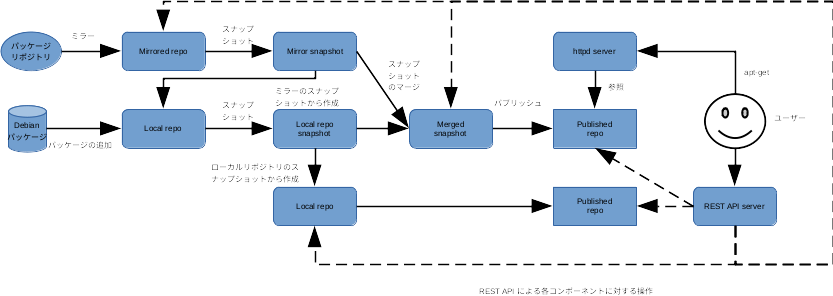
\includegraphics[width=1.0\hsize]{image202005/aptly-image00.png}

\begin{itemize}
\item $B%_%i!<%j%]%8%H%j$OB>$N%Q%C%1!<%8%j%]%8%H%j$+$i:n@.$7$^$9!#(B
\item  $B%m!<%+%k%Q%C%1!<%8$O%Q%C%1!<%8$rDI2C$9$k$+!"%m!<%+%k%_%i!<$+$i:n@.$G$-$^$9!#(B
\item  $B:n@.$7$?%m!<%+%k%_%i!<$d%m!<%+%k%j%]%8%H%j$O$=$N$^$^$G$O%Q%C%1!<%8%j%]%8%H%j$H$7$F$OMxMQ$G$-$:!"%Q%V%j%C%7%e(B($B8x3+(B)$B$9$kI,MW$,$"$j$^$9!#(B
\item  $B%m!<%+%k%_%i!<$d%m!<%+%k%j%]%8%H%j$O%9%J%C%W%7%g%C%H$r:n@.$G$-$^$9!#(B
\item  $B%9%J%C%W%7%g%C%H$+$i%9%J%C%W%7%g%C%H$b:n@.$G$-!"%9%J%C%W%7%g%C%HF1;N$N0MB84X78$b%a%?%G!<%?$H$7$F;}$A$^$9!#(B
\item  $B%9%J%C%W%7%g%C%HF1;N$G%^!<%8$G$-$^$9!#(B
\item  $B%Q%W%j%C%7%e$7$?%Q%C%1!<%8%j%]%8%H%j$O(B aptly $B$GDs6!$5$l$k(B http$B%5!<%P!<$r;HMQ!"$^$?$O$=$NB>(Bhttp$B%5!<%P!<$r;H$C$F8x3+$G$-$^$9!#(B
\end{itemize}

\subsubsection{aptly $B$r;HMQ$9$k:]$KCm0U$9$k$3$H(B}

aptly $B$G$O%Q%C%1!<%8%j%]%8%H%j$r8x3+$9$k>l9g$K!"(BGnuPG$B$K$h$k=pL>$,I,MW$H$J$j$^$9(B($BI,?\$G$O$J$/!"%*%W%7%g%s$G=pL>$*$h$S(B
$B3NG'$rL5;k$G$-$^$9(B)$B!#(Baptly $B$O0lEY%m!<%+%k$K%Q%C%1!<%8$H%a%?>pJs$rJ]B8$7!"(B
$B$=$l$i$rAH$_9g$o$;$F!"%Q%C%1!<%8%j%]%8%H%j$KI,MW$J%a%?%G!<%?(B (Release$B%U%!%$%k$J$I(B)$B$r:F9=C[(B
$B$7$^$9!#:F9=C[$7$?%a%?%G!<%?$O%U%k%_%i!<$G$"$C$F$bFbMF$,0[$J$k$?$a!"@5$7$/%Q%C%1!<%8%j%]%8%H%j(B
$B$r1?MQ$9$k$K$O$3$l$i$K(B GnuPG $B$K$h$k=pL>$,I,MW$K$J$j$^$9!#(B
$B%a%?%G!<%?$r4^$a$?%U%k%_%i!<$r9=C[$7$?$$>l9g$O(B archvsync (\url{https://salsa.debian.org/mirror-team/archvsync}) 
$B$d(B apt-mirror $B%Q%C%1!<%8$r;H$&$HNI$$$G$7$g$&!#(B

$B$^$?%Q%C%1!<%8%j%]%8%H%j$N9=C[$K$O%O!<%I%j%s%/$r;H$$$^$9!#$h$C$F%O!<%I%j%s%/$N@)8B$,E,MQ$5$l$k$3$H$KCm0U(B
$B$,I,MW$G$9!#(BAmazon S3 $B$J$I$N%/%i%&%I%9%H%l!<%8$K%Q%C%1!<%8%j%]%8%H%j$r%Q%V%j%C%7%e$9$k:]$K$O$3$N@)8B$O$"$j$^$;$s!#(B

$B0J2<$+$i$O!"(Baptly $B$K;H$$J}$K$D$$$F@bL@$7$^$9!#(B

\subsection{aptly $B$N%$%s%9%H!<%k(B}

aptly$B$O8x<0(BDebian$B%Q%C%1!<%8$H$7$FDs6!$5$l$F$$$^$9!#<9I.;~$N(BDebian$B%Q%C%1!<%8%P!<%8%g%s$O(B 1.3.0+ds1-4 $B$H$J$C$F$$$^$9!#(B
$B0J2<$N%3%^%s%I$G%$%s%9%H!<%k$G$-$^$9!#(B

\begin{commandline}
$ sudo apt update
$ sudo apt install aptly
\end{commandline}

$B$^$?(B Upstream $B$N%P!<%8%g%s$O(B 1.4.0 $B$H$J$C$F$*$j!"(BGnuPG 2.x $B$X$N%5%]!<%H6/2=$J$I$,9T$o$l$F$$$^$9!#(B
$B:G?7%P!<%8%g%s$r;H$$$?$$>l9g$K$O!"0J2<$N$h$&$K%"%C%W%9%H%j!<%`(B $B$,Ds6!$9$k%j%]%8%H%j$GDs6!$5$l$F$$$k(B
$B%Q%C%1!<%8$,MxMQ$G$-$^$9!#(B $B%G%#%9%H%j%S%e!<%7%g%sIt$,(B squeeze $B$H$J$C$F$$$^$9$,!"0l$D$N%G%#%9%H%j%S%e!<%7%g%s(B
$B$N$_$GDs6!$5$l$F$$$k$N$G!"5$$K$7$J$/$F$bNI$$$G$9!#(B

\begin{commandline}
$ wget -qO - https://www.aptly.info/pubkey.txt | sudo apt-key add -
$ sudo sh -c "echo deb http://repo.aptly.info/ squeeze main > /etc/apt/sources.list.d/aptly.list"
$ sudo apt update
$ sudo apt install aptly
\end{commandline}

\subsubsection{aptly $B$N@_Dj(B}

aptly $B$N@_Dj$O(B \$HOME/.aptly.conf$B$K5-:\$5$l$F$$$^$9!#(B
$BFbMF$O(B aptly config $B%3%^%s%I$N(B show $B%5%V%3%^%s%I$G3NG'$G$-$^$9!#(B
$B$b$A$m$sIaCJ$*;H$$$N%(%G%#%?Ey$G3NG'$7$F$b$+$^$$$^$;$s!#(B

\begin{commandline}
$ aptly config show
{
    "rootDir": "/home/aptly/.aptly",
    "downloadConcurrency": 4,
    "downloadSpeedLimit": 0,
    "architectures": [],
    "dependencyFollowSuggests": false,
    "dependencyFollowRecommends": false,
    "dependencyFollowAllVariants": false,
    "dependencyFollowSource": false,
    "dependencyVerboseResolve": false,
    "gpgDisableSign": false,
    "gpgDisableVerify": false,
    "gpgProvider": "gpg",
    "downloadSourcePackages": false,
    "skipLegacyPool": true,
    "ppaDistributorID": "ubuntu",
    "ppaCodename": "",
    "skipContentsPublishing": false,
    "FileSystemPublishEndpoints": {},
    "S3PublishEndpoints": {},
    "SwiftPublishEndpoints": {}
}
\end{commandline}

$B>\:Y$O>J$-$^$9$,!"=EMW$J$N$O(B rootDir $B$N9`L\$G!"$3$3$G;XDj$5$l$k%G%#%l%/%H%j$K(Baptly $B$,4IM}$9$k(B
$B%Q%C%1!<%8$N%a%?%G!<%?$d%m!<%+%k%Q%C%1!<%8%j%]%8%H%jEy$,3JG<$5$l$^$9!#(B
$B$^$?(B Amazon S3$B$d(B OpenStack Swift  $B$X$N%"%C%W%m!<%I$r9T$&:]$K$O!"(BS3PublishEndpoints$B$d(BSwiftPublishEndpoints$B$KBP$7$F(B
$B%"%/%;%9%-!<Ey$r@_Dj$7$^$9!#(B
$B3F9`L\$N>\:Y$O(B Configuration (\url{https://www.aptly.info/doc/configuration/}) $B$r3NG'$7$F$/$@$5$$!#(B

\subsection{GnuPG $B80$N:n@.$H%Q%C%1!<%8%j%]%8%H%j$N=pL>3NG'I,MW$J8x3+80$N%$%s%]!<%H(B}

aptly $B$r;H$&A0$K!"(BGnuPG$B80$N:n@.$H!"%Q%C%1!<%8%_%i!<85$N(BGnuPG$B8x3+80$r%$%s%]!<%H$9$k(B
$BI,MW$,$"$j$^$9!#(B
$BA0=R$7$?$h$&$K!"@5$7$/%Q%C%1!<%8%j%]%8%H%j$r1?MQ$9$k$K$O(BGnuPG$B$K$h$k=pL>$,I,MW$J$?$a!"(B
GnuPG$B80$r:n@.$7$^$9!#4{$K(BGnuPG$B80$r;}$C$F$$$k>l9g$b!"%j%]%8%H%j4IM}MQ$KJLES(BGnuPG$B80$r(B
$B:n@.$7$F$*$/$H$h$$$G$7$g$&!#(BGnuPG$B80$N:n@.$K$O0J2<$N$h$&$K<B9T$7$^$9!#(B

\begin{commandline}
$ gpg --gen-key

<$BCfN,(B>

$BK\L>(B: aptly
$BEE;R%a!<%k!&%"%I%l%9(B: aptly@example.com
$B<!$N%f!<%6(BID$B$rA*Br$7$^$7$?(B:
    "aptly <aptly@example.com>"

<$BCfN,(B>
$B8x3+80$HHkL)80$r:n@.$7!"=pL>$7$^$7$?!#(B

pub   rsa3072 2020-05-01 [SC] [$BM-8z4|8B(B: 2022-05-01]
      E67BDF3221F4CDFD47F4A3639A64752708B70EFA
uid                      aptly <aptly@example.com>
sub   rsa3072 2020-05-01 [E] [$BM-8z4|8B(B: 2022-05-01]
\end{commandline}

$B<!$K%Q%C%1!<%8%_%i!<85$N(B GnuPG$B8x3+80$r%$%s%]!<%H$7$^$9!#(B
$B%Q%C%1!<%8%j%]%8%H%j$N%_%i!<85$N>pJs$r<hF@$9$k:]$K%_%i!<85$N=pL>$r3NG'$9$kI,MW$,$"$k$?$a$G$9!#(B
Debian $B$N%*%U%#%7%c%k%Q%C%1!<%8%j%]%8%H%j$r;H$&>l9g$K$O0J2<$N$h$&$K<B9T$7$^$9!#(B

\begin{commandline}
$ sudo apt install debian-archive-keyring
$ gpg --no-default-keyring --keyring /usr/share/keyrings/debian-archive-keyring.gpg --export | \
        gpg --no-default-keyring --keyring trustedkeys.gpg --import
\end{commandline}

$B<!$K(B Debian $B$GDs6!$5$l$F$$$k%Q%C%1!<%8$r;H$C$F$$$k?M$O!"(BGnuPG v2 $B$G:n@.$7$?80$r(B v1 $B$K%3%s%P!<%H(B
$B$9$kI,MW$,$"$j$^$9!#$3$l$O(B Debian $B$N%Q%C%1!<%8$,(B GnuPG v1 $B$K0MB8$7$F$$$k$?$a$G$9!#(B
$B8x3+80(B E67BDF3221F4CDFD47F4A3639A64752708B70EFA $B$r%3%s%P!<%H$7!"(BGnuPG v1 $B$K%$%s%]!<%H$9$kJ}K!$r(B
$B0J2<$K<($7$^$9!#(B

\begin{commandline}
$ gpg --output gpg2_export_pub.gpg --armor --export E67BDF3221F4CDFD47F4A3639A64752708B70EFA
$ gpg --output gpg2_export_sec.gpg --armor --export-secret-key E67BDF3221F4CDFD47F4A3639A64752708B70EFA
$ gpg1 --import gpg2_export_pub.gpg
gpg: $B80(B08B70EFA: $B8x3+80(B"aptly <aptly@example.com>"$B$r%$%s%]!<%H$7$^$7$?(B
gpg:           $B=hM}?t$N9g7W(B: 1
gpg:             $B%$%s%]!<%H(B: 1  (RSA: 1)
gpg: $B:G>.$N!V$"$kDxEY$N?.MQ!W(B3$B!":G>.$N!VA4LLE*?.MQ!W(B1$B!"(BPGP$B?.MQ%b%G%k(B
gpg: $B?<$5(B: 0  $BM-8z@-(B:   1  $B=pL>(B:   0  $B?.MQ(B: 0-, 0q, 0n, 0m, 0f, 1u
gpg: $B<!2s$N?.MQ%G!<%?%Y!<%98!::$O!"(B2022-05-01$B$G$9(B
$ gpg1 --import --allow-secret-key-import gpg2_export_sec.gpg
gpg: $B80(B08B70EFA: $BHkL)80$r%$%s%]!<%H$7$^$7$?(B
gpg: $B80(B08B70EFA:"aptly <aptly@example.com>"$BJQ99$J$7(B
gpg:           $B=hM}?t$N9g7W(B: 1
gpg:               $BJQ99$J$7(B: 1
gpg:       $BHkL)80$NFI$_9~$_(B: 1
gpg:     $BHkL)80$N%$%s%]!<%H(B: 1
\end{commandline}

$B$^$?:n@.$9$k%Q%C%1!<%8%j%]%8%H%j$K%"%/%;%9$9$k%^%7%s$K%Q%C%1!<%8%j%]%8%H%j$N8x3+80$rEPO?$9$k$3$H$r(B
$BK:$l$J$$$h$&$K$7$^$7$g$&!#8x3+80$N=PNOJ}K!$H=PNO$7$?8x3+80$rEPO?$9$kJ}K!$r0J2<$K<($7$^$9!#(B

\begin{commandline}
$ gpg --export --armor > aptly.pub
\end{commandline}

\begin{commandline}
$ sudo apt-key add aptly.pub
\end{commandline}

\subsection{$B%Q%C%1!<%8%_%i!<%j%]%8%H%j$N:n@.(B}

$B%m!<%+%k$K%Q%C%1!<%8%_%i!<%j%]%8%H%j$r:n@.$9$k>l9g!"(B aptly mirror $B%3%^%s%I$N(B create $B%5%V%3%^%s%I$r;HMQ$7$^$9!#(B
$B%3%^%s%I$K%m!<%+%k$GMxMQ$9$kL>A0(B(name)$B!"%j%]%8%H%j$N(BURL$B!"%G%#%9%H%j%S%e!<%7%g%s!"%3%s%]!<%M%s%H$r;XDj$7$^$9!#(B
$BNc$($P!"(B

\begin{itemize}
	\item $BL>A0(B: debian-buster
	\item $B%j%]%8%H%j(BURL: http://deb.debian.org/debian/
	\item $B%G%#%9%H%j%S%e!<%7%g%s(B: buster
	\item $B%3%s%]!<%M%s%H(B: main
	\item $B%"!<%-%F%/%A%c(B: $B$9$Y$F(B
\end{itemize}

$B>e5-$N$h$&$J%Q%C%1!<%8%_%i!<%j%]%8%H%j$r:n@.$9$k>l9g!"0J2<$N$h$&$K<B9T$7$^$9!#(B
$B<B9T$9$k$H%j%]%8%H%j$,=i4|2=$5$l$^$9!#(B


\begin{commandline}
$ aptly mirror create debian-buster http://deb.debian.org/debian/ buster main
\end{commandline}

$B:n@.$7$?%Q%C%1!<%8%_%i!<%j%]%8%H%j$N>pJs$O(B list $B%5%V%3%^%s%I$G(B
$B3NG'$G$-$^$9!#(B

\begin{commandline}
$ aptly mirror list
List of mirrors:
 * [debian-buster]: http://deb.debian.org/debian/ buster

To get more information about mirror, run `aptly mirror show <name>`.
\end{commandline}

$B$^$?>\:Y$J>pJs$,I,MW$J>l9g$O(B show $B%5%V%3%^%s%I$G3NG'$G$-$^$9!#(B

\begin{commandline}
$ aptly mirror show debian-buster
Name: debian-buster
Archive Root URL: http://deb.debian.org/debian/
Distribution: buster
Components: main
Architectures: amd64, arm64, armel, armhf, i386, mips, mips64el, mipsel, ppc64el, s390x
Download Sources: no
Download .udebs: no
Last update: never

Information from release file:
Acquire-By-Hash: yes
Architectures: amd64 arm64 armel armhf i386 mips mips64el mipsel ppc64el s390x
Changelogs: http://metadata.ftp-master.debian.org/changelogs/@CHANGEPATH@_changelog
Codename: buster
Components: main contrib non-free
Date: Sat, 09 May 2020 09:51:02 UTC
Description:  Debian 10.4 Released 09 May 2020

Label: Debian
Origin: Debian
Suite: stable
Version: 10.4
\end{commandline}

$B$^$@$3$N>uBV$G$O%j%]%8%H%j$N%a%?%G!<%?$d%Q%C%1!<%8$,$J$$>uBV$N$?$a!"%_%i!<85$+$i<hF@$9$kI,MW$,$"$j$^$9!#(B
$B<hF@$9$k$K$O(B update $B%5%V%3%^%s%I$r<B9T$7$^$9!#(B
$B<B9T$9$k$H%a%?%G!<%?$r<hF@$7!"%Q%C%1!<%8$N%_%i!<$r3+;O$7$^$9!#(B

\begin{commandline}
$ aptly mirror update debian-buster
\end{commandline}

$B>e5-$G$O;XDj$7$?%G%#%9%H%j%S%e!<%7%g%s$N%3%s%]!<%M%s%H$r$9$Y$F%_%i!<$7$^$9!#(B
$BFCDj$N%"!<%-%F%/%A%c$N$_$d!"%_%i!<$7$?$$%Q%C%1!<%8$r;XDj$7$?$$>l9g$K$O!"%*%W%7%g%s$r;H$&$3$H$G(B
$B@)8f$G$-$^$9!#0J2<$G$O$h$/MxMQ$5$l$k%*%W%7%g%s$r0J2<$K<($7$^$9!#(B

\begin{itemize}
	\item $B%"!<%-%F%/%A%c$r;XDj$9$k(B: -architectures
	\item $B%Q%C%1!<%8$r%U%#%k%?!<$9$k(B: -filter
	\item $B%U%#%k%?!<$G;XDj$5$l$?%Q%C%1!<%8$K0MB8$9$k%Q%C%1!<%8$b%_%i!<$9$k(B: -filter-with-deps
	\item $B%=!<%9%Q%C%1!<%8$b%_%i!<$9$k(B: -with-sources
\end{itemize}

$B%"!<%-%F%/%A%c$r(Bamd64 $B$H(B arm64$B!"%_%i!<$9$k%Q%C%1!<%8$r(B busybox$B!"0MB8$9$k%Q%C%1!<%8$H%=!<%9%Q%C%1!<%8$b%_%i!<$9$k>l9g(B
$B$K$O0J2<$N$h$&$K<B9T$7$^$9!#(B

\begin{commandline}
$ aptly mirror create -architectures=amd64,arm64 -filter='busybox' \
    -filter-with-deps -with-sources busybox-mirror http://deb.debian.org/debian/ buster main
\end{commandline}

$B<B9T$7!"<hF@$7$?%Q%C%1!<%8$O(B \$HOME/.aptly $B%G%#%l%/%H%j0J2<$KJ]B8$5$l$^$9!#(B
$B%U%!%$%k$NG[CV$O(B git $B%j%]%8%H%j$N(B git object $B$N$h$&$JG[CV$K$J$C$F$$$^$9!J(Bsha265sum $BCM!K!#(B

\begin{commandline}
.aptly
$B('(!(!(B db
$B("(B $B('(!(!(B 000004.ldb
$B("(B $B('(!(!(B 000007.ldb
$B("(B $B('(!(!(B 000008.log
$B("(B $B('(!(!(B CURRENT
$B("(B $B('(!(!(B LOCK
$B("(B $B('(!(!(B LOG
$B("(B $B(&(!(!(B MANIFEST-000009
$B(&(!(!(B pool
    $B('(!(!(B 1b
    $B("(B $B(&(!(!(B 00
    $B("(B     $B(&(!(!(B f7cef567645a7e695caf6c1ad395_gcc-8-base_8.3.0-6_amd64.deb
    $B('(!(!(B 1e
    $B("(B $B(&(!(!(B 32
    $B("(B     $B(&(!(!(B ea742bddec4ed5a530ee2f423cdf_busybox_1.30.1-4_amd64.deb
<$B>JN,(B> 
\end{commandline}

$B:n@.$7$?%_%i!<$GDs6!$5$l$k%Q%C%1!<%8$r3NG'$9$k$K$O(B aptly mirror $B%3%^%s%I$N(B search $B%5%V%3%^%s%I;HMQ$7$^$9!#(B
$B8!:w$9$k%_%i!<L>$H8!:wMQ$N%/%(%j!<$r;XDj$7!"<B9T$7$^$9!#0J2<$K(B $B%Q%C%1!<%8L>$,(B busy\* $B!"%"!<%-%F%/%A%c$,(B
arm64 $B$G$"$k%Q%C%1!<%8$r8!:w$9$k$K$O0J2<$N$h$&$K<B9T$7$^$9!#8!:wMQ%/%(%j!<$r;XDj$7$J$$>l9g$ODs6!$5$l$k%Q(B
$B%C%1!<%8$,A4$F=PNO$5$l$^$9!#(B

\begin{commandline}
$ aptly mirror search busybox-mirror 'Name (% busy*), $Architecture (arm64)'
busybox_1:1.30.1-4_arm64
busybox-static_1:1.30.1-4_arm64
\end{commandline}

\subsection{$B%m!<%+%k%Q%C%1!<%8%j%]%8%H%j$N:n@.(B}

$B%m!<%+%k%Q%C%1!<%8%j%]%8%H%j$O!"FH<+$G:n@.$7$?%Q%C%1!<%8$r%j%]%8%H%j$G4IM}$7$?$$>l9g$J$I$K;HMQ$7$^$9!#(B
$B$^$:4IM}$9$k$?$a$N%j%]%8%H%j$r:n@.$9$kI,MW$,$"$j$^$9!#(B
$B%j%]%8%H%j$r:n@.$9$k$K$O!"(Baptly repo $B%3%^%s%I(B $B$N(Bcreate $B%5%V%3%^%s%I$K:n@.$9$k%j%]%8%H%jL>$r;XDj$7$F<B9T$7$^$9!#(B
$B$3$N%j%]%8%H%jL>$O(B Debian $B%Q%C%1!<%8$GMxMQ$5$l$k(B $B%G%#%9%H%j%S%e!<%7%g%sL>(B (unstable, buster $B$J$I(B)
$B$HI3IU$1$i$l$F$$$^$9!#(B

\begin{commandline}
$ aptly repo create my-repo
\end{commandline}

$B$^$?%m!<%+%k%j%]%8%H%j$r:n@.$9$k>l9g!"%9%J%C%W%7%g%C%H$+$i$b:n@.$G$-$^$9!#(B

\begin{commandline}
$ aptly repo create my-repo from snapshot snapshot-name
\end{commandline}

\subsubsection{$B%m!<%+%k%Q%C%1!<%8%j%]%8%H%j$X$N%Q%C%1!<%8$NDI2C(B}

create $B%5%V%3%^%s%I$G:n@.$7$?CJ3,$G$O!"%m!<%+%k%Q%C%1!<%8%j%]%8%H%j$K$^$@%Q%C%1!<%8$,EPO?$5$l$F$$$J$$>uBV$J$N$G!"(B
$B%Q%C%1!<%8$rDI2C$7$^$9!#DI2C$9$kJ}K!$O0J2<$NJ}K!$,$"$j$^$9!#(B

\subsubsubsection{add $B%5%V%3%^%s%I$r;H$C$?%Q%C%1!<%8$NDI2C(B}

add $B%5%V%3%^%s%I$O(B $BFCDj$N(Bdebian $B%P%$%J%j%Q%C%1!<%8!"$^$?$O(Bdsc (Debian source packages control file)$B$r85$K%=!<%9%Q%C%1!<%8$rDI2C(B
$B$7$?$$>l9g$KMxMQ$7$^$9!#(B
$B%Q%C%1!<%8$r;XDj$7$F%m!<%+%k%Q%C%1!<%8%j%]%H%j$KDI2C$7$?$$>l9g$O!"(Badd $B%5%V%3%^%s%I$K%Q%C%1!<%8%U%!%$%k$N%Q%9$r;XDj$7$F<B9T$7$^$9!#(B

\begin{commandline}
$ aptly repo add my-repo pool/liblz4-1_1.9.2-2_amd64.deb
Loading packages...
[+] liblz4-1_1.9.2-2_amd64 added
\end{commandline}

$B$^$?%=!<%9%Q%C%1!<%8$rDI2C$7$?$$>l9g$K$O(B dsc $B%U%!%$%k$r;XDj$7$F<B9T$7$^$9!#(B

\begin{commandline}
$ aptly repo add my-repo pool/lz4_1.9.2-2.dsc
Loading packages...
[+] lz4_1.9.2-2_source added
\end{commandline}

$BFCDj$N%G%#%l%/%H%j$K$"$k%Q%C%1!<%8$9$Y$FDI2C$7$?$$>l9g$K$OBP>]$N%G%#%l%/%H%j$r;XDj$9$l$P$h$$$G$9!#(B

\begin{commandline}
$ aptly repo add my-repo pool
Loading packages...
[+] liblz4-1-dbgsym_1.9.2-2_amd64 added
[+] liblz4-1_1.9.2-2_amd64 added
[+] liblz4-dev_1.9.2-2_amd64 added
[+] liblz4-tool_1.9.2-2_all added
[+] lz4-dbgsym_1.9.2-2_amd64 added
[+] lz4_1.9.2-2_source added
[+] lz4_1.9.2-2_amd6 added
\end{commandline}

add $B%3%^%s%I$r;H$C$?>l9g!"%U%!%$%k$N%5%$%:$d%U%!%$%k%O%C%7%eCM$N3NG'$O9T$o$l$J$$$?$aCm0U$,I,MW$G$9!#(B
$B$h$j0BA4$K%Q%C%1!<%8$r%j%]%8%H%j$KDI2C$7$?$$>l9g!"<!$G@bL@$9$k(B include $B%5%V%3%^%s%I$r;H$$$^$9!#(B

\subsubsubsection{include $B%5%V%3%^%s%I$r;H$C$?%Q%C%1!<%8$NDI2C(B}

$B%m!<%+%k%Q%C%1!<%8%j%]%8%H%j$X$N%Q%C%1!<%8$NDI2C$K$O(B add $B%5%V%3%^%s%I$NB>$K(Binclude $B%5%V%3%^%s%I$bMxMQ2DG=$G$9!#(B
add $B%5%V%3%^%s%I$H$N0c$$$O=hM}$NBP>]$,(B .changes $B%U%!%$%k$G$"$k;v$G$9!#(B
.changes $B%U%!%$%k$r;XDj$7$F<B9T$9$k$K$O0J2<$N$h$&$K<B9T$7$^$9!#<B9T$9$k$H!"(B.changes $B%U%!%$%k$K5-:\$5$l$F$$$k%Q%C%1!<%8(B
$B$,EPO?$5$l$^$9!#FC$K;XDj$7$J$$>l9g!"<B9T8e$K$O%Q%C%1!<%8%U%!%$%kEy$O:o=|$5$l$F$7$^$&$N$G!":o=|$7$?$/$J$$>l9g$K$O(B
-no-remove-files $B%*%W%7%g%s$r;XDj$9$kI,MW$,$"$j$^$9!#(B
$B$^$?(B.changes $B$K(BGnuPG$B$K$h$k=pL>$r9T$C$F$*$i$:!"=pL>$NM-L5$rL5;k$7$?$$>l9g$K$O(B -accept-unsigned $B%*%W%7%g%s$r(B
$B;XDj$9$kI,MW$,$"$j$^$9!#(B

\begin{commandline}
Format: 1.8
Date: Tue, 12 Nov 2019 07:58:47 +0900
Source: lz4

<$BCfN,(B>

Checksums-Sha1:
 44348438b55dc32132df8039513a57c4c1cd87a5 1073 lz4_1.9.2-2.dsc
 3790bc3c9e6d4e26e5063855cf847f5af91d8420 12712 lz4_1.9.2-2.debian.tar.xz
 ce4d29ed984de507203d917e671c1894c9778e8c 323008 liblz4-1-dbgsym_1.9.2-2_amd64.deb
 aed6d84f4636d37cd94b90e9ce0320dee853eca6 57148 liblz4-1_1.9.2-2_amd64.deb
 018ef0f8bf34411b4b928072f5c1f2d1abf8103f 76752 liblz4-dev_1.9.2-2_amd64.deb
 bf32ee9eee03ef69d6b0526bed92dcc95af57883 5088 liblz4-tool_1.9.2-2_all.deb
 39f1aa1950030608ad528a4f4fe951b37e0e4956 410216 lz4-dbgsym_1.9.2-2_amd64.deb
 dec576464d1c5e4b2b69e59ab29208f4e6d741eb 6648 lz4_1.9.2-2_amd64.buildinfo
 689287ecea701b76f99c5d30040ca584bdc58fde 84076 lz4_1.9.2-2_amd64.deb

<$B>JN,(B>
\end{commandline}
 
\begin{commandline}
$ aptly repo include -repo my-repo pool/lz4_1.9.2-2_amd64.changes
Loading repository my-repo for changes file lz4_1.9.2-2_amd64.changes...
[+] liblz4-1-dbgsym_1.9.2-2_amd64 added
[+] liblz4-1_1.9.2-2_amd64 added
[+] liblz4-dev_1.9.2-2_amd64 added
[+] liblz4-tool_1.9.2-2_all added
[+] lz4-dbgsym_1.9.2-2_amd64 added
[+] lz4_1.9.2-2_source added
[+] lz4_1.9.2-2_amd64 added
\end{commandline}
%<!-- $ aptly repo include -repo my-repo -no-remove-files -accept-unsigned pool/lz4_1.9.2-2_amd64.changes -->

$B>e5-$G$O<B9T$9$k:]$K!"(B-repo $B%*%W%7%g%s$G%j%]%8%H%jL>$r;XDj$7$F$$$^$9!#(B
$B$3$l$O(B changelog $B$G;XDj$5$l$F$$$k%G%#%9%H%j%S%e!<%7%g%sL>(B(unstable $B$J$I(B)$B$,%j%]%8%H%jL>$H9gCW$7$J$$>l9g(B
$B$K%(%i!<$K$J$k$?$a$G$9!#(B

$B$^$?%G%#%l%/%H%j$r;XDj$9$k>l9g$K$O!"(B.changes $B$,3JG<$5$l$F$$$k%G%l%/%H%j$r;XDj$7$^$9!#(B

\begin{commandline}
$ aptly repo include -repo my-repo pool
Loading repository my-repo for changes file lz4_1.9.2-2_amd64.changes...
[+] liblz4-1-dbgsym_1.9.2-2_amd64 added
[+] liblz4-1_1.9.2-2_amd64 added
[+] liblz4-dev_1.9.2-2_amd64 added
[+] liblz4-tool_1.9.2-2_all added
[+] lz4-dbgsym_1.9.2-2_amd64 added
[+] lz4_1.9.2-2_source added
[+] lz4_1.9.2-2_amd64 added
\end{commandline}

$B;XDj$7$?%G%#%l%/%H%j$K(B .changes $B%U%!%$%k$,$J$$>l9g$d!"(B.changes $B$NFbMF$,0[$J$k>l9g$K$O(B
$B=hM}$5$l$^$;$s!#(B

\begin{commandline}
$ aptly repo include -repo my-repo -no-remove-files -accept-unsigned pool
[!] unable to process file lz4_1.9.2-2_amd64.changes: size mismatch: expected 12712 != obtained 12568 
[!] Some files were skipped due to errors:
  pool/lz4_1.9.2-2_amd64.changes
ERROR: some files failed to be added
\end{commandline}


% $B%j%]%8%H%j$N%"%C%W%m!<%@!<$r8GDj$7$?$$>l9g$O(B**-uploaders-file=**$B$r;H$&!#(B
% uploaders $B$N%U%)!<%^%C%H$O(B https://www.aptly.info/doc/aptly/repo/include/ $B$K=q$$$F$"$k!#(B

\subsubsubsection{$B%m!<%+%k%_%i!<$+$i$NDI2C(B}

aptly mirror $B%3%^%s%I$K$h$C$F:n@.$7$?%m!<%+%k%_%i!<$GDs6!$5$l$F$$$k%Q%C%1!<%8$b(B
$B%m!<%+%k%j%]%8%H%j$KDI2C$G$-$^$9!#$3$N>l9g(B import $B%5%V%3%^%s%I$rMxMQ$7$^$9!#(B

$BNc$($P!"%m!<%+%k%_%i!<(B busybox-mirror $B$K$"$k(B busybox $B$G;O$^$k%Q%C%1!<%8$r(B my-repo $B%m!<%+%k(B
$B%j%]%8%H%j$KDI2C$9$k>l9g$K$O0J2<$N$h$&$K<B9T$7$^$9!#(B

\begin{commandline}
$ aptly repo import busybox-mirror my-repo busybox
Loading packages...
[o] busybox_1:1.30.1-4_source imported
[o] busybox-static_1:1.30.1-4_amd64 imported
[o] busybox_1:1.30.1-4_arm64 imported
[o] busybox_1:1.30.1-4_amd64 imported
[o] busybox-static_1:1.30.1-4_arm64 imported
\end{commandline}

Package Queries(\url{https://www.aptly.info/doc/feature/query/})
$B$K%Q%C%1!<%8L>$N;XDjJ}K!Ey$K4X$9$k@bL@$,$"$k$N$G6=L#$N$"$kJ}$O;2>H$7$F$/$@$5$$!#(B

\subsubsection{$B%m!<%+%k%Q%C%1!<%8%j%]%8%H%j$N:o=|(B}

$B%m!<%+%k%Q%C%1!<%8%j%]%8%H%j$N>pJs$r:o=|$7$?$$>l9g$K$O!"(Bdrop $B%5%V%3%^%s%I$K:o=|$7$?$$%j%]%8%H%jL>$r;XDj$7$^$9!#(B

\begin{commandline}
$ aptly repo drop my-repo
\end{commandline}

\subsubsection{$B$=$NB>%m!<%+%k%j%]%8%H%j$K4X$9$kA`:n(B}

\begin{itemize}
\item repo list

  $B:n@.$5$l$?%j%]%8%H%j$N%j%9%H$r=PNO$7$^$9!#(B

\item repo copy

  $B%j%]%8%H%j$K$"$k%Q%C%1!<%8$r;XDj$7$?%j%]%8%H%j$K%3%T!<$7$^$9!#(B
  $B%3%T!<@h$N%j%]%8%H%j$O@h$K:n@.$7$F$*$/I,MW$,$"$kE@$KCm0U$,I,MW$G$9!#(B

\begin{commandline}
  $ aptlu repo create my-repo-next
  $ aptly repo copy my-repo my-repo-next 'Name (%lib*)'
  Loading packages...
  [o] liblz4-tool_1.9.2-2_all copied
  [o] liblz4-1_1.9.2-2_amd64 copied
  [o] liblz4-1-dbgsym_1.9.2-2_amd64 copied
  [o] liblz4-dev_1.9.2-2_amd64 copied
\end{commandline}

\item repo move

  $B%j%]%8%H%j$K$"$k%Q%C%1!<%8$r;XDj$7$?%j%]%8%H%j$K0\F0$7$^$9!#(B
  $B%3%T!<@h$N%j%]%8%H%j$O@h$K:n@.$7$F$*$/I,MW$,$"$kE@$KCm0U$,I,MW$G$9!#(B

\item repo remove

  $B;XDj$7$?%Q%C%1!<%8$r%j%]%8%H%j$+$i:o=|$7$^$9!#(B

\item repo search

  $B%j%]%8%H%j$GDs6!$5$l$F$$$k%Q%C%1!<%8$r8!:w$7$^$9!#(B

\item repo edit

  $B%j%]%8%H%j$K4X$9$k>pJs$r=$@5$7$^$9!#(B

\item repo rename

  $B%j%]%8%H%jL>$rJQ99$7$^$9!#(B

\end{itemize}

\subsection{$B%9%J%C%W%7%g%C%H(B}

aptly mirror update $B%3%^%s%I$r<B9T$7$?>l9g!"%_%i!<85$N%Q%C%1!<%8>pJsEy$H40A4$KF14|$9$k$?$a!"(B
$B%_%i!<85$G:o=|$5$l$?%Q%C%1!<%8$O%m!<%+%k%_%i!<$G$b:o=|$5$l!"99?7$5$l$?%Q%C%1!<%8$b8E$$$b$N$O(B
$B;D$C$F$$$J$$>uBV$K$J$C$F$7$^$$$^$9!#(B
$B$^$?%m!<%+%k%Q%C%1!<%8%j%]%8%H%j$G$b1?MQ$K$h$C$F$O>e5-$HFa$8$h$&$J$3$H$,5/$3$k2DG=@-$b(B
$B$"$j$^$9!#$3$N$h$&$J;v$,5/$-$F$b:$$i$J$$$h$&$K$9$k$?$a$K!"%9%J%C%W%7%g%C%H$r:n@.$7!"(B
$B%Q%C%1!<%8$N9=@.$r0];}$G$-$k$h$&4IM}$7$^$9!#(B

\subsubsection{$B%9%J%C%W%7%g%C%H$N:n@.$H3NG'(B}

$B%9%J%C%W%7%g%C%H$r:n@.$9$k$K$O!"(Baptly snapshot $B%3%^%s%I$N(B create $B%5%V%3%^%s%I$r;HMQ$7$^$9!#(B
$BNc$($P!"%m!<%+%k%_%i!<(B buster-mirror $B$N%9%J%C%W%7%g%C%H$r(B buster-mirror-2020512 $B$H$7$F:n@.$9$k$K$O(B
$B0J2<$N$h$&$K<B9T$7$^$9!#(B

\begin{commandline}
$ aptly snapshot create buster-mirror-2020512 from mirror buster-mirror
\end{commandline}

$B%9%J%C%7%g%C%H$O(B $B%m!<%+%k%j%]%8%H%j$+$i$b:n@.$G$-$^$9!#(B
$B%m!<%+%k%j%]%8%H%j(B my-repo $B$N%9%J%C%W%7%g%C%H$r(B my-repo-20200512 $B$H$7$F:n@.$9$k$K$O0J2<$N$h$&$K(B
$B<B9T$7$^$9!#(B

\begin{commandline}
$ aptly snapshot create imy-repo-20200510 from repo my-repo
\end{commandline}

$B8=:_:n@.$5$l$F$$$k%9%J%C%W%7%g%C%H$r3NG'$9$k$K$O(B list $B%5%V%3%^%s%I!"(B
$B%9%J%C%W%7%g%C%H$N>pJs$r3NG'$9$k$K$O$O(B show $B%5%V%3%^%s%I$r;H$$$^$9!#(B

\begin{commandline}
$ aptly snapshot list
List of snapshots:
 * [busybox-buster-mirror-20200512]: Snapshot from mirror [busybox-buster-mirror]: http://deb.debian.org/debian/ buster
 * [my-repo-20200512]: Snapshot from local repo [my-repo]

To get more information about snapshot, run `aptly snapshot show <name>`.
$ aptly snapshot show my-repo-20200512
Name: my-repo-20200512
Created At: 2020-05-15 07:06:32 UTC
Description: Snapshot from local repo [my-repo]
Number of packages: 12
Sources:
  my-repo [local]
\end{commandline}

\subsubsection{$B%9%J%C%W%7%g%C%H$N%^!<%8(B}

$B:n@.$7$?%9%J%C%W%7%g%C%H$r%^!<%8$7!"?7$7$$%9%J%C%W%7%g%C%H$r:n@.$9$k$K$O(B merge $B%5%V%3%^%s%I$r;H$$$^$9!#(B
$B:n@.$7$?$$%9%J%C%W%7%g%C%HL>$K%^!<%8$9$k%9%J%C%W%7%g%C%H$r;XDj$7$^$9!#(B

\begin{commandline}
$ aptly snapshot merge my-product-release-20200512 my-repo-20200512 busybox-buster-mirror-20200512

Snapshot my-product-release-20200512 successfully created.
You can run 'aptly publish snapshot my-product-release-20200512' to publish snapshot as Debian repository.
$ aptly snapshot list
List of snapshots:
 * [busybox-buster-mirror-20200512]: Snapshot from mirror [busybox-buster-mirror]: http://deb.debian.org/debian/ buster
 * [my-product-release-20200512]: Merged from sources: 'my-repo-20200512', 'busybox-buster-mirror-20200512'
 * [my-repo-20200512]: Snapshot from local repo [my-repo]

To get more information about snapshot, run `aptly snapshot show <name>`.

$ aptly snapshot show my-product-release-20200512
Name: my-product-release-20200512
Created At: 2020-05-15 07:20:35 UTC
Description: Merged from sources: 'my-repo-20200512', 'busybox-buster-mirror-20200512'
Number of packages: 15
Sources:
  my-repo-20200512 [snapshot]
  busybox-buster-mirror-20200512 [snapshot]
\end{commandline}

\subsubsection{$B%9%J%C%W%7%g%C%H$N8!>Z(B}

$B%9%J%C%W%7%g%C%H$N>uBV$K$h$C$F$O%Q%C%1!<%8$N0MB84X78$,0];}$G$-$F$J$$>l9g$,$"$j$^$9!#(B
$B$3$l$O%Q%C%1!<%8$NDI2C$7K:$l$d!"%m!<%+%k%_%i!<%j%]%8%H%j$r(B
$B9=C[$7$?:]$K(B -filter-with-deps $B%*%W%7%g%s$rIU$1$F$$$J$+$C$?$3$H$J$I$,860x$H$J$j$^$9!#(B
$B$3$N$h$&$J>uBV$r3NG'$9$k$?$a$K!"%9%J%C%W%7%g%C%HFbMF$r8!>Z$9$k%5%V%3%^%s%I(B verify $B$,(B
$BMQ0U$5$l$F$$$^$9!#(B
$B0J2<$G$O!"(B-filter-with-deps $B$rIU$1$:$K(B busybox$B$+$i;O$^$k%Q%C%1!<%8$N%_%i!<$r:n@.$7!"(B
$B$=$N%9%J%C%W%7%g%C%H$r8!>Z$7$?7k2L$G$9!#$3$N%9%J%C%W%7%g%C%H$G$O(B libc6 (>= 2.28) $B$,(B
$BITB-$7$F$$$k$3$H$,$o$+$j$^$9!#(B

\begin{commandline}
$ aptly mirror create -architectures=amd64 -filter='busybox' \
    busybox-buster-mirror-without-dep http://deb.debian.org/debian/ buster main
$ aptly mirror update busybox-buster-mirror-without-dep
$ aptly snapshot create busybox-buster-mirror-without-dep-v1 from mirror busybox-buster-mirror-without-dep
$ aptly snapshot verify busybox-buster-mirror-without-dep-v1
Loading packages...
Verifying...
Missing dependencies (1):
  libc6 (>= 2.28) [amd64]
\end{commandline}

$B$3$N$h$&$J>l9g!"B-$j$J$$%Q%C%1!<%8$rDs6!$9$k%j%b!<%H%Q%C%1!<%8%j%]%8%H%j$r(B apt-line $B$KDI2C$9$k$J$I$GBP1~$G$-$^$9$,!"(B
$B$3$N%j%b!<%H%Q%C%1!<%8%j%]%8%H%j$NFbMF$,JQ99$5$l$k2DG=@-$b9M$($i$l$^$9!#:,K\E*$KLdBj$r2sHr$9$k$?$a$K$O!"F1$8%9%J%C%W%7%g%C%H(B
$BFb$GDs6!$G$-$k$h$&$K$7$?$[$&$,$h$$$G$7$g$&!#(B
$B%9%J%C%W%7%g%C%H$N%Y!<%9$H$J$C$?%_%i!<$r(B -filter-with-deps $BIU2C$7$?8e99?7$7!":FEY%9%J%C%W%7%g%C%H$r:n@.$9$k$+!"(B
$BB>$N%9%J%C%W%7%g%C%H$GI,MW$H$9$k%Q%C%1!<%8$,Ds6!$5$l$F$$$k$J$i!"<!$G@bL@$9$k(B pull $B%5%V%3%^%s%I$r;H$C$F!"B>$N%9%J%C%W%7%g%C%H$+$i(B
$B%Q%C%1!<%8$r<h$j9~$`$3$H$b$G$-$^$9!#(B

\begin{commandline}
$ aptly mirror edit -filter-with-deps busybox-buster-mirror-without-dep
$ aptly mirror show busybox-buster-mirror | grep '^Filter With Deps'
Filter With Deps: yes
$ aptly mirror update busybox-buster-mirror
\end{commandline}

\subsubsubsection{$BB>$N%9%J%C%W%7%g%C%H$+$i%Q%C%1!<%8$r<h$j9~$_!"?7$7$$%9%J%C%W%7%g%C%H$r:n@.$9$k(B}

$B4{B8$N%9%J%C%W%7%g%C%H$K!"B>$N%9%J%C%W%7%g%C%H$GDs6!$5$l$k%Q%C%1!<%8$r<h$j9~$_!"?7$7$$%9%J%C%W%7%g%C%H(B
$B$r:n@.$9$k$K$O!"(Bpull $B%5%V%3%^%s%I$r;H$$$^$9!#(B
$B%Y!<%9$H$9$k%9%J%C%W%7%g%C%H(B busybox-buster-mirror-without-dep-v1 $B$K(B $B%9%J%C%W%7%g%C%H(B libc-dev-mirror-20200512 $B$G(B
$BDs6!$5$l$k(B libc6 $B%Q%C%1!<%8$r<h$j9~$_!"%9%J%C%W%7%g%C%H(B busybox-buster-mirror-v1 $B$r:n@.$9$k$K$O!"0J2<$N$h$&$K<B9T(B
$B$7$^$9!#(B

\begin{commandline}
$ aptly snapshot pull busybox-buster-mirror-without-dep-v1 libc-dev-mirror-20200512 busybox-buster-mirror-v1 libc6
Dependencies would be pulled into snapshot:
    [busybox-buster-mirror-without-dep-v1]: Snapshot from mirror [busybox-buster-mirror-without-dep]: \
	http://deb.debian.org/debian/ buster
from snapshot:
    [libc-dev-mirror-20200512]: Snapshot from mirror [libc-dev-mirror]: http://deb.debian.org/debian/ buster
and result would be saved as new snapshot busybox-buster-mirror-v1.
Loading packages (8)...
Building indexes...
[+] gcc-8-base_8.3.0-6_amd64 added
[+] libc6_2.28-10_amd64 added
[+] libgcc1_1:8.3.0-6_amd64 added

Snapshot busybox-buster-mirror-v1 successfully created.
You can run 'aptly publish snapshot busybox-buster-mirror-v1' to publish snapshot as Debian repository.
\end{commandline}

$B?7$7$/:n@.$5$l$?%9%J%C%W%7%g%C%H(B busybox-buster-mirror-v1 $B$r3NG'$9$k$H!"(Blibc6 $B%Q%C%1!<%8$H(Blibc6$B$K0MB8$9$k%Q%C%1!<%8(B
$B$,<h$j9~$^$l!"(Bverify $B%5%V%*%W%7%g%s$N7k2L$bLdBj$J$$$3$H$,$o$+$j$^$9!#(B

\begin{commandline}
$ aptly snapshot show -with-packages busybox-buster-mirror-v1
Name: busybox-buster-mirror-v1
Created At: 2020-05-15 18:13:45 UTC
Description: Pulled into 'busybox-buster-mirror-without-dep-v1' with 'libc-dev-mirror-20200512' as source, \
	pull request was: 'libc6'
Number of packages: 5
Sources:
  busybox-buster-mirror-without-dep-v1 [snapshot]
  libc-dev-mirror-20200512 [snapshot]
Packages:
  busybox_1:1.30.1-4_amd64
  busybox-static_1:1.30.1-4_amd64
  gcc-8-base_8.3.0-6_amd64
  libc6_2.28-10_amd64
  libgcc1_1:8.3.0-6_amd64
$ aptly snapshot verify busybox-buster-mirror-v1
Loading packages...
Verifying...
All dependencies are satisfied.
\end{commandline}

\subsubsubsection{$B%9%J%C%W%7%g%C%H$N:o=|(B}

$B%9%J%C%W%7%g%C%H$r:o=|$9$k>l9g!"(Bdrop $B%5%V%3%^%s%I$r;HMQ$7$^$9!#(B
$B:o=|$9$k%9%J%C%W%7%g%C%H$,B>$N%9%J%C%W%7%g%C%H$G%^!<%8$5$l$F$$$k>l9g$K$O:o=|$5$l$^$;$s!#(B
-force $B%*%W%7%g%s$G6/@)E*$K:o=|$b$G$-$^$9$,!"%j%]%8%H%j$N@09g@-$,$J$/$J$k2DG=@-$,$"$k$N$G!"(B
$B%^!<%8@h$N%9%J%C%W%7%g%C%H$r:o=|$7$F$+$i!":o=|$9$k$h$&$K$7$^$9!#(B
$B2<5-$N<B9TNc$G$O!"%9%J%C%W%7%g%C%H(B my-repo-20200512 $B$O(B $B%9%J%C%W%7%g%C%H(B my-product-release-20200512
$B$K0MB8$5$l$F$$$k$?$a!":o=|$G$-$^$;$s!#(B
\begin{commandline}
$ aptly snapshot drop my-repo-20200512
Snapshot `my-repo-20200512` was used as a source in following snapshots:
 * [my-product-release-20200512]: Merged from sources: 'my-repo-20200512', 'busybox-buster-mirror-20200512'
ERROR: won't delete snapshot that was used as source for other snapshots, use -force to override
\end{commandline}

$B$b$7%9%J%C%W%7%g%C%H(B my-repo-20200512 $B$r:o=|$7$?$$>l9g$K$O!"0MB8$5$l$F$$$k(B my-product-release-20200512$B$r(B
$B@h$K:o=|$9$kI,MW$,$"$j$^$9!#(B

\begin{commandline}
$ aptly snapshot drop my-product-release-20200512
Snapshot `my-product-release-20200512` has been dropped.
$ aptly snapshot drop my-repo-20200512
Snapshot `my-repo-20200512` has been dropped.
\end{commandline}

\subsubsubsection{$B%9%J%C%W%7%g%C%H$K4X$9$kB>$N5!G=(B}
\begin{itemize}
\item diff

  $B%9%J%C%W%7%g%C%H4V$N:9J,$r=PNO$7$^$9!#(B

\item search 

  $B;XDj$7$?%9%J%C%W%7%g%C%H$GDs6!$5$l$F$$$k%Q%C%1!<%8$r8!:w$7$^$9!#(B

\item rename

  $B%9%J%C%W%7%g%C%HL>$rJQ99$7$^$9!#(B

\end{itemize}

\subsection{$B%j%]%8%H%j$N8x3+(B($B%Q%V%j%C%7%e(B)}

$B$3$l$^$G%m!<%+%k%_%i!<$d%m!<%+%k%j%]%8%H%j!"%9%J%C%W%7%g%C%H$K$D$$$F@bL@$7$F$-$^$7$?$,!"(B
$B$3$l$^$G$N>uBV$G$O$^$@(B apt-line $B$H$7$F;2>H$G$-$k%Q%C%1!<%8%j%]%8%H%j$K$O$J$C$F$$$J$$$?$a!"(B
apt $B%3%^%s%IEy$G%Q%C%1!<%8$N%@%&%m!<%I$d%$%s%9%H!<%k$O$G$-$^$;$s!#(Bpublish $B%3%^%s%I$rMQ$$$F(B
$B%Q%C%1!<%8%j%]%8%H%j$r8x3+$9$kI,MW$,$"$j$^$9!#(B

$B8x3+$9$k%Q%C%1!<%8%j%]%8%H%j$O%9%J%C%W%7%g%C%H$H%m!<%+%k%Q%C%1!<%8%j%]%8%H%j$+$i:n@.$G$-$^$9$,!"(B
$B8e<T$O?d>)$5$l$^$;$s!#$3$NM}M3$H$7$F!"%m!<%+%k%Q%C%1!<%8%j%]%8%H%j$O%9%J%C%W%7%g%C%H$H$O0[$J$j!"(B
$BFbMF$,JQ99$5$l$k2DG=@-$,$"$k$?$a$G$9!#0J2<$G$O%9%J%C%W%7%g%C%H$r%Q%C%1!<%8%j%]%8%H%j$H$7$F(B
$B8x3+$9$kJ}K!$r@bL@$7$^$9!#(B

\subsubsection{$B%9%J%C%W%7%g%C%H$+$i%Q%C%1!<%8%j%]%8%H%j$r:n@.$9$k(B}

$B%9%J%C%W%7%g%C%H(B my-product-release-20200512 $B$r%Q%C%1!<%8%j%]%8%H%j$H$7$F8x3+$9$k>l9g!"(B
snapshot $B%5%V%3%^%s%I$K%9%J%C%W%7%g%C%HL>$r;XDj$7$F<B9T$7$^$9!#<B9T$9$k$H(B GnuPG $B=pL>(B
$B$9$k$K%Q%9%U%l!<%:$rMW5a$5$l$^$9!#(B

\begin{commandline}
$ aptly publish snapshot my-product-release-20200512 
Loading packages...
Generating metadata files and linking package files...
Finalizing metadata files...
Signing file 'Release' with gpg, please enter your passphrase when prompted:

$B<!$N%f!<%6$NHkL)80$N%m%C%/$r2r=|$9$k$K$O(B
$B%Q%9%U%l!<%:$,$$$j$^$9(B:"aptly <aptly@example.com>"
3072$B%S%C%H(BRSA$B80(B, ID 08B70EFA$B:n@.F|IU$O(B2020-05-10

Clearsigning file 'Release' with gpg, please enter your passphrase when prompted:

$B<!$N%f!<%6$NHkL)80$N%m%C%/$r2r=|$9$k$K$O(B
$B%Q%9%U%l!<%:$,$$$j$^$9(B:"aptly <aptly@example.com>"
3072$B%S%C%H(BRSA$B80(B, ID 08B70EFA$B:n@.F|IU$O(B2020-05-10

Snapshot my-product-release-20200512 has been successfully published.
Please setup your webserver to serve directory '/home/aptly/.aptly/public' with autoindexing.
Now you can add following line to apt sources:
  deb http://your-server/ buster main
  deb-src http://your-server/ buster main
Don't forget to add your GPG key to apt with apt-key.

You can also use `aptly serve` to publish your repositories over HTTP quickly.
\end{commandline}
 
$B%Q%C%1!<%8%j%]%8%H%j$O(B \$(HOME)/.aptly/public $B0J2<$K:n@.$5$l$^$9!#(B
$BBP>]%G%#%l%/%H%j$r(Bapt-line $B$G;2>H$G$-$k$h$&$K@_Dj$9$k$H!"(Bapt $B%3%^%s%IEy$+$i%Q%C%1!<%8$r<hF@$G$-$k(B
$B$h$&$K$J$j$^$9!#(B
$B$^$?>e5-=PNO$K$"$k$h$&$K(B apt-line $B$G@_Dj$9$kFbMF$r%G%#%9%H%j%S%e!<%7%g%sL>$,(B buster $B$K$J$C$F$$$^$9!#(B
$B$3$l$O(B $B%9%J%C%W%7%g%C%H(B my-product-release-20200512 $B$N%Y!<%9$,(B Debian $B%_%i!<$N(B buster $B%G%#%9%H%j(B
$B%S%e!<%7%g%s$@$C$?$?$a$G$9!#%G%#%9%H%j%S%e!<%7%g%sL>$rJQ99$7$?$$>l9g$K$O!"(B-distribution $B%*%W%7%g%s$r(B
$B;H$$$^$9!#(B

\begin{commandline}
$ aptly publish snapshot -distribution="my-product" my-product-release-20200512 
<$B>JN,(B>

Now you can add following line to apt sources:
  deb http://your-server/ my-product main
  deb-src http://your-server/ my-product main
\end{commandline}

\subsubsection{$B%Q%C%1!<%8%j%]%8%H%j$N99?7(B}

$B%Q%C%1!<%8%j%]%8%H%jFbMF$r!"?7$7$/:n@.$7$?%9%J%C%W%7%g%C%H$K99?7$7$?$$>l9g!"(Bswitch $B%5%V%3%^%s%I$r;H$$$^$9!#(B
$B0J2<$G$O!"(Bzlib1g $B%Q%C%1!<%8$r4^$s$@%9%J%C%W%7%g%C%H$r%^!<%8$7$?(B $B%9%J%C%W%7%g%C%H(B my-product-release-20200513
$B$K99?7$7$F$$$^$9!#(B

\begin{commandline}
$ aptly mirror drop zlib-buster-mirror
$ aptly mirror create -architectures=amd64 -filter='zlib1g' -filter-with-deps zlib-buster-mirror \
	http://deb.debian.org/debian/ buster main
$ aptly mirror update zlib-buster-mirror
$ aptly snapshot create zlib-buster-mirror-20200512 from mirror zlib-buster-mirror
$ aptly snapshot merge my-product-release-20200513 my-repo-20200512 busybox-buster-mirror-20200512 zlib-buster-mirror-20200512
$ aptly snapshot diff my-product-release-20200512 my-product-release-20200513
  Arch   | Package | Version in A | Version in B
+ amd64  | zlib1g  | -            | 1:1.2.11.dfsg-1
$ aptly publish switch my-product my-product-release-20200513
Loading packages...
Generating metadata files and linking package files...
Finalizing metadata files...
Signing file 'Release' with gpg, please enter your passphrase when prompted:

<$B>JN,(B>
\end{commandline}

\subsubsection{$B8x3+$5$l$F$$$k%Q%C%1!<%8%j%]%8%H%j$N3NG'(B}

$B8x3+$5$l$F$$$k%Q%C%1!<%8%j%]%8%H%j$r3NG'$9$k$K$O(B list $B%5%V%3%^%s%I$r;H$$$^$9!#(B
$B$3$l$K$h$j8x3+$5$l$F$$$k%Q%C%1!<%8%j%]%8%H%j$,$I$N%9%J%C%W%7%g%C%H!&%m!<%+%k%Q%C%1!<%8%j%]%8%H%j$K0MB8$7$F$$$k$N$+(B
$B3NG'$G$-$^$9!#(B

\begin{commandline}
$ aptly publish list
Published repositories:
  * ./buster [amd64, source] publishes {main: [my-product-release-20200512]: Merged from sources: \
	'my-repo-20200512', 'busybox-buster-mirror-20200512'}
  * ./my-product [amd64, source] publishes {main: [my-product-release-20200513]: Merged from sources: \
	'my-repo-20200512', 'busybox-buster-mirror-20200512', 'zlib-buster-mirror-20200512'}
\end{commandline}

$B%Q%C%1!<%8%j%]%8%H%j$G%5%]!<%H$7$F$$$k%"!<%-%F%/%A%c$J$I$b3NG'$7$?$$>l9g$K$O(B show $B%5%V%3%^%s%I$r;H$$$^$9!#(B

\begin{commandline}
$ aptly publish show my-product
Prefix: .
Distribution: my-product
Architectures: amd64 source
Sources:
  main: my-product-release-20200513 [snapshot]
\end{commandline}

\subsubsection{$B%Q%C%1!<%8%j%]%8%H%j$N:o=|(B}

$B%Q%C%1!<%8%j%]%8%H%j$r:o=|$9$k$K$O(B drop $B%5%V%3%^%s%I$r;H$$$^$9!#(B
$B<B9T$9$k$H%Q%C%1!<%8%j%]%8%H%j=PNO@h%G%#%l%/%H%j$b:o=|$5$l$^$9!#(B

\begin{commandline}
$ aptly publish drop buster
$ aptly publish list
Published repositories:
  * ./my-product [amd64, source] publishes {main: [my-product-release-20200513]: Merged from sources: \
	'my-repo-20200512', 'busybox-buster-mirror-20200512', 'zlib-buster-mirror-20200512'}
\end{commandline}

\subsubsection{$B%Q%C%1!<%8%j%]%8%H%j$X$N%"%/%;%9(B}

$B%Q%V%j%C%7%e$7$?%Q%C%1!<%8%j%]%8%H%j$GDs6!$5$l$k%Q%C%1!<%8$rMxMQ$9$k$K$O!"0J2<$N(B3$B$D$NJ}K!$,$"$j$^$9!#(B

\begin{enumerate}
	\item File $B%W%m%H%3%k$r;HMQ$7$F!"(B.aptly/public/ $B$r(Bapt-line $B$KDI2C$9$k!#(B
	\item aptly $B$GDs6!$5$l$k(B http $B%5!<%P!<$rN)$A>e$2!"(Bhttp $B7PM3$G<hF@$9$k!#(B
	\item $BJLES(B HTTP $B%5!<%P!<$rN)$A>e$2!"(B.aptly/public/$B$r;2>H$9$k$h$&@_Dj$7!"(Bhttp $B7PM3$G<hF@$9$k!#(B
\end{enumerate}

$B3F!9$NJ}K!$r0J2<$K@bL@$7$^$9!#(B

\subsubsubsection{File $B%W%m%H%3%k$r;H$&(B}

File $B%W%m%H%3%k$r;H$&>l9g$K$O!"(Bapt-line $B$K(B $B%Q%C%1!<%8%j%]%8%H%j$r;XDj$7$^$9!#(B
$B$3$N>l9g!"%Q%C%1!<%8%j%]%8%H%j$rDs6!$7$F$$$k%^%7%s0J30$+$i$O%"%/%;%9$G$-$J$$E@$KCm0U$,I,MW$G$9!#(B

\begin{commandline}
$ sudo sh -c "echo deb file:///home/aptly/.aptly/public/ my-product main" >> /etc/apt/sources.list.d/my-product.list
$ sudo apt update
\end{commandline}

\subsubsubsection{aptly $B$GDs6!$5$l$k(B http $B%5!<%P!<;H$&(B}

aptly $B$GDs6!$5$l$k(B http $B%5!<%P!<$r;H$&$K$O!"(Baptly serve $B%3%^%s%I$r;H$$$^$9!#(B
$B<B9T$9$k$H(B $B%Q%C%1!<%8%j%]%8%H%j$X(B8080$BHV%]!<%H7PM3$G%"%/%;%9$G$-$k$h$&$K$J$j$^$9!#(B

\begin{commandline}
$ aptly serve
Serving published repositories, recommended apt sources list:

# ./my-product [amd64, source] publishes {main: [my-product-release-20200513]: Merged from sources: 'my-repo-20200512', \
	'busybox-buster-mirror-20200512', 'zlib-buster-mirror-20200512'}
deb http://ryzen7:8080/ my-product main
deb-src http://ryzen7:8080/ my-product main

Starting web server at: :8080 (press Ctrl+C to quit)...
\end{commandline}

$B$=$N8e%"%/%;%9$9$k%^%7%s$K(B apt-line $B$rDI2C$9$k$3$H$G!"%Q%C%1!<%8%j%]%8%H%j$K%"%/%;%9$G$-$k$h$&$K$J$j$^$9!#(B
\begin{commandline}
$ sudo sh -c "echo deb http://ryzen7:8080/ my-product main" > /etc/apt/sources.list.d/my-product.list
$ sudo apt update
\end{commandline}

$B%"%/%;%9$9$k$?$a$N%]!<%H$d%[%9%HL>$r;XDj$7$?$$>l9g$K$O(B -listen $B%*%W%7%g%s$r;H$$$^$9!#(B
$B%m!<%+%k%k!<%W%P%C%/%"%I%l%9(B 127.0.0.1 $B$N(B 8888$BHV%]!<%H$H$7$F5/F0$7$?$$>l9g$K$O0J2<$N$h$&$K<B9T$7$^$9!#(B
\begin{commandline}
$ aptly serv -listen=127.0.0.1:8888
\end{commandline}

\subsubsubsection{$BJLES(B $B%Q%C%1!<%8%j%]%8%H%jMQ(B http $B%5!<%P!<$rN)$A>e$2$k(B}

nginx $B$rNc$K(B http $B%5!<%P!<$N@_DjJ}K!$r@bL@$7$^$9!#(B
nginx $B$r%$%s%9%H!<%k$7!"(B/etc/nginx/sites-available/apt $B$r:n@.$7$^$9!#(B

\begin{commandline}
$ sudo apt-get install nginx
$ sudo vi /etc/nginx/sites-available/apt
\end{commandline}

\begin{commandline}
server {
    listen 80; 
    listen [::]:80;
 
    server_name aptly.exaple.com;
    root /var/www-apt;
    allow all;
    autoindex on; 
 
    # Full access for everybody for the stable debian repo
    location /public {
        root /home/aptly/.aptly;
        allow all;
    }
 
    # Allow access to the top level to be able to download the GPG key 
    location / { 
        allow all;
    }
}
\end{commandline}

/etc/nginx/sites-enabled/apt $B$K%7%s%\%j%C%/%j%s%/$r:n@.$7!"(Bnginx $B$r:F5/F0$7$^$9!#(B
\begin{commandline}
$ sudo ln -s /etc/nginx/sites-available/apt /etc/nginx/sites-enabled/apt
$ sudo systemctl restart nginx
\end{commandline}

$B$=$N8e%"%/%;%9$9$k%^%7%s$K(B apt-line $B$rDI2C$9$k$3$H$G!"%Q%C%1!<%8%j%]%8%H%j$K%"%/%;%9$G$-$k$h$&$K$J$j$^$9!#(B
\begin{commandline}
$ sudo sh -c "echo deb http://ryzen/public/ my-product main" > /etc/apt/sources.list.d/my-product.list
$ sudo apt update
\end{commandline}

\subsection{REST API}

aptly $B$O(B REST API $B$,Ds6!$5$l$F$*$j!"(BAPI $BMQ%5!<%P!<$rN)$A>e$2$k$3$H$GMxMQ$G$-$k$h$&$K$J$j$^$9!#(B
API $B%5!<%P!<$N5/F0$O(B aptly api $B%3%^%s%I$N(B serve $B%5%V%*%W%7%g%s$r<B9T$7$^$9!#(B

\begin{commandline}
$ aptly api serve
Starting web server at: :8080 (press Ctrl+C to quit)...
[GIN-debug] [WARNING] Now Gin requires Go 1.6 or later and Go 1.7 will be required soon.
...
\end{commandline}

$B5/F0$7$?8e$O!"%5!<%P!<$KBP$7$F(B API $B$r<B9T$G$-$k$h$&$K$J$j$^$9!#(B
repo$B!"(Bsnapshot$B!"(Bpublish$B!"(Bpackage$B!"(Bgraph $B$K4X$9$k(BAPI$B$,Ds6!$5$l$F$*$j!"(B
mirror $B$d(B db $B$KBP$9$k(B API $B$O$^$@Ds6!$5$l$F$$$^$;$s!#(B
API $B$N>\:Y$O(B Web $B%5%$%H$N(BAPI (\url{https://www.aptly.info/doc/api/})$B$K5-:\$5$l$F$$$^$9!#(B
$B$3$3$G$O(B API $B$N;H$$J}$r$$$/$D$+>R2p$7$^$9!#(B

\begin{itemize}
  \item $B%m!<%+%k%Q%C%1!<%8%j%]%8%H%j$GDs6!$5$l$F$$$k%Q%C%1!<%80lMw$r<hF@$9$k!#(B

\begin{commandline}
$ curl http://localhost:8080/api/repos/my-repo/packages
["Pamd64 lz4 1.9.2-2 76bbfff77a824848","Pamd64 lz4-dbgsym 1.9.2-2 e71a271edd2c351","Psource lz4 1.9.2-2 91576aff056e5141",\
	"Pall liblz4-tool 1.9.2-2 8db5a921d2f58813","Pamd64 liblz4-1 1.9.2-2 30f3b73d9c877f6b",\
	"Pamd64 liblz4-1-dbgsym 1.9.2-2 7a9c4cd5844174f8","Pamd64 liblz4-dev 1.9.2-2 9f649d10440c4c7f"]
\end{commandline}

 \item $B%9%J%C%W%7%g%C%H$K4X$9$k>pJs$r<hF@$9$k!#(B

\begin{commandline}
$ curl http://localhost:8080/api/snapshots
[{"Name":"busybox-buster-mirror-20200512","CreatedAt":"2020-05-15T19:29:25.376281727Z",\
	"Description":"Snapshot from mirror [busybox-buster-mirror]: http://deb.debian.org/debian/ buster","Origin":"Debian",\
	"NotAutomatic":"","ButAutomaticUpgrades":""},
	{"Name":"busybox-buster-mirror-without-dep-v1","CreatedAt":"2020-05-15T18:09:04.530501686Z",\
	"Description":"Snapshot from mirror [busybox-buster-mirror-without-dep]: http://deb.debian.org/debian/ buster",
	"Origin":"Debian","NotAutomatic":"","ButAutomaticUpgrades":""},
	{"Name":"my-product-release-20200512","CreatedAt":"2020-05-15T21:51:09.772154566Z",\
	"Description":"Merged from sources: 'my-repo-20200512', 'busybox-buster-mirror-20200512'","Origin":"",
	"NotAutomatic":"", "ButAutomaticUpgrades":""}, \
	{"Name":"my-product-release-20200513","CreatedAt":"2020-05-15T19:38:33.373419548Z", \
	"Description":"Merged from sources: 'my-repo-20200512', 'busybox-buster-mirror-20200512', 
	'zlib-buster-mirror-20200512'", "Origin":"","NotAutomatic":"","ButAutomaticUpgrades":""}, \
	{"Name":"my-repo-2* Connection #0 to host localhost left intact 0200512","CreatedAt":"2020-05-15T19:29:26.185504839Z", \
	"Description":"Snapshot from local repo [my-repo]","Origin":"","NotAutomatic":"","ButAutomaticUpgrades":""}, \
	{"Name":"zlib-buster-mirror-20200512","CreatedAt":"2020-05-15T19:29:25.510882855Z", \
	"Description":"Snapshot from mirror [zlib-buster-mirror]: http://deb.debian.org/debian/ buster","Origin":"Debian"," \
	NotAutomatic":"","ButAutomaticUpgrades":""}]
\end{commandline}

 \item $B%m!<%+%k%Q%C%1!<%8%j%]%8%H%j(B my-repo $B$N%9%J%C%W%7%g%C%H(B $B$r(B my-repo-devel $B$H$7$F:n@.$9$k(B

\begin{commandline}
$ curl -X POST -H 'Content-Type: application/json' --data '{"Name":"my-repo-devel"}' \
	http://localhost:8080/api/repos/my-repo/snapshots
{"Name":"my-repo-devel","CreatedAt":"2020-05-16T09:44:46.985707235+09:00", \
	"Description":"Snapshot from local repo [my-repo]","Origin":"","NotAutomatic":"","ButAutomaticUpgrades":""}
\end{commandline}

\end{itemize}

\subsubsection{REST API $B$r07$&%=%U%H%&%'%"(B}

REST API $B$OD>@\07$$$E$i$$$?$a!"(BPython $B$d(B Ruby $B$J$I$N%W%m%0%i%_%s%08@8l$GA`:n$7$?$$$H;W$&?M$,$[$H$s$I$@$H;W$$$^$9!#(B
aptly $B$r07$&%D!<%k$d(BAPI$B%i%C%Q!<$r>R2p$7$^$9!#(B

\begin{itemize}
  \item Python
    \begin{itemize}
    \item aptly-api-client / \url{https://github.com/gopythongo/aptly-api-client}
    \item python-aptly / \url{https://github.com/tcpcloud/python-aptly}
    \item, pyaptly / \url{https://github.com/adfinis-sygroup/pyaptly}
    \end{itemize}

  \item Ruby
    \begin{itemize}
    \item aptly\_cli / \url{https://github.com/sepulworld/aptly_cli}
    \item aptly-simple / \url{https://github.com/serge-name/aptly-simple}
    \item aptlier / \url{https://github.com/3ofcoins/aptlier}
    \end{itemize}

  \item shell
    \begin{itemize}
    \item  nitrux-repository-util / \url{(https://github.com/Nitrux/nitrux-repository-util}
    \end{itemize}
\end{itemize}

\subsection{$B$^$H$a(B}

Debian$B%Q%C%1!<%8%j%]%8%H%j$NE}9g%D!<%k$G$"$k(B aptly $B$N;H$$J}$r>R2p$7$^$7$?!#(B
API$B$N5!G=$O$^$@B-$j$F$J$$ItJ,$bB?$/!";H$$$E$i$$$H$3$m$O$"$j$^$9$,!"(B
dpkg-dev $B$d(B apt-ftparchive $B;H$$$J$,$i(BCI/CD$B4D6-$r9=C[$5$l$F$$$kJ}$O$b$A$m$s!"(B
$B2q<R$N%$%s%U%i@0Hw$d(BDebian/Ubuntu$B$r$D$+$C$?@=IJ3+H/$r$5$l$F$$$kJ}$d(BDebian$B%Q%C%1!<%8(B
$B%a%s%F%J$K$bM-MQ$J%D!<%k$G$9!#$3$l$r5!2q$K(B aptly $B$X$N$-$j$+$($r8!F$$7$F$_$^$;$s$+!#(B

% $B:};R$K$9$k$?$a$K!"(B4$B$NG\?t$K$9$kI,MW$,$"$k!#(B
% $B$=$N$?$a$ND4@0(B
\dancersection{$B%a%b(B}{}
\mbox{}\newpage
\mbox{}\newpage

\vspace*{15cm}
\hrule
\vspace{2mm}

\includegraphics[width=2cm]{image200502/openlogo-nd.eps}
\noindent \Large \bf Debian $BJY6/2q;qNA(B\\
\noindent \normalfont \debmtgyear{}$BG/(B\debmtgmonth{}$B7n(B\debmtgdate{}$BF|(B \hspace{5mm}  $B=iHGBh(B1$B:~H/9T(B\\
\noindent \normalfont $BEl5~%(%j%"(B Debian $BJY6/2q(B $B!JJT=8!&0u:~!&H/9T!K(B\\
\hrule
\end{document}
